\documentclass[tikz,border=5pt]{standalone}

\usepackage{tikz}
%\usetikzlibrary{calc}
\usepackage{stix2}
\usepackage{amsmath}
\usepackage{amsthm}
\usepackage{amssymb}
\usepackage{xcolor}



\definecolor{azul}{RGB}{0, 60, 113}
\definecolor{dorado}{RGB}{196, 151, 57}
\definecolor{morado}{RGB}{101, 43, 145}
\definecolor{rosa}{RGB}{146, 33, 209}
\definecolor{azulC}{RGB}{52, 90, 229}


\begin{document}

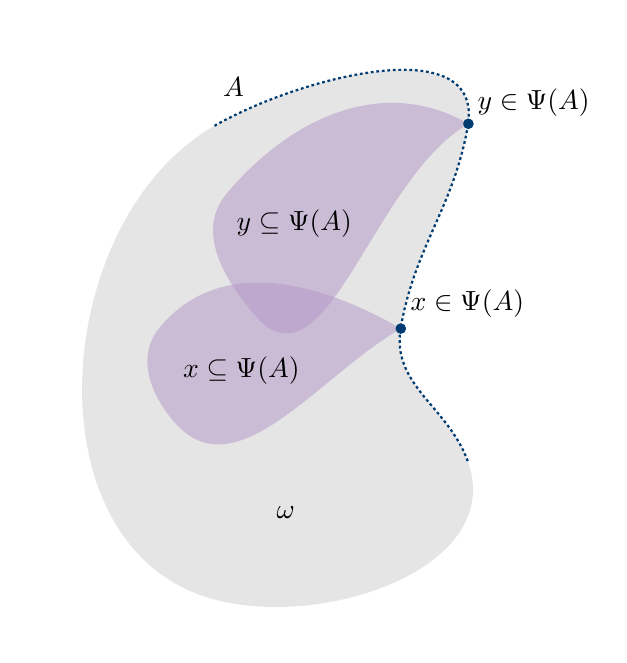
\begin{tikzpicture}[scale=1.7]
    \fill[gray!20]
    (0,-.5)
    to[out=80,in=260] (.5,1)
    to[out=260+180,in=30] (-1.4,1)
    to[out=30+180,in=160] (-1.5,-2.5)
    to[out=160+180,in=290] (.5,-1.5)
    to[out=290+180,in=80+180] (0,-.5);

    \fill[fill=morado!50, fill opacity=0.5]
    (0,-.51)
    to[out=80+70,in=50] (-1.8,-.5)
    to[out=50+180,in=130] (-1.7,-1.2)
    to[out=130+180,in=-80-70] (0,-.51);

    \fill[fill=morado!50, fill opacity=0.5]
    (.505,1.02)
    to[out=80+70,in=50] (-1.3,0.5)
    to[out=50+180,in=130] (-1.1,-.4)
    to[out=130+180,in=-80-70] (.505,1.02);

    %\draw[morado, line width=.4]
    %(0,-.51)
    %to[out=80+70,in=50] (-1.8,-.5)
    %to[out=50+180,in=130] (-1.7,-1.2)
    %to[out=130+180,in=-80-70] (0,-.51);
    \node[above right] at (-1.7,-1) {$x \subseteq  \Psi(\mathscr{A})$};

    %\draw[morado, line width=.4]
    %(.505,1.02)
    %to[out=80+70,in=50] (-1.3,0.5)
    %to[out=50+180,in=130] (-1.1,-.4)
    %to[out=130+180,in=-80-70] (.505,1.02);
    \node[above right] at (-1.3,.1) {$y \subseteq  \Psi(\mathscr{A})$};
    
    \draw[thick, dash pattern=on 1pt off 1pt on 1pt off 1pt, azul]
    (.5,-1.5)
    to[out=290+180,in=80+180] (0,-.5)
    to[out=80,in=260] (.5,1)
    to[out=260+180,in=30] (-1.4,1);
    \node[above right] at (-1.4,1.15) {$\mathscr{A}$};

    \draw[fill=azul, azul] (0,-.51) circle (1pt);
    \node[above right] at (0,-.5) {$x \in \Psi(\mathscr{A})$};

    \draw[fill=azul, azul] (.505,1.02) circle (1pt);
    \node[above right] at (.5,1) {$y \in \Psi(\mathscr{A})$};


    \node[above right] at (-1,-2) {$\omega$};
\end{tikzpicture}

\end{document}